\documentclass[a4paper,12pt]{report}

\usepackage{alltt, fancyvrb, url}
\usepackage{graphicx}
\usepackage[utf8]{inputenc}
\usepackage{hyperref}
\usepackage{array}
\usepackage[table]{xcolor}

% Questo commentalo se vuoi scrivere in inglese.
\usepackage[italian]{babel}

\usepackage[italian]{cleveref}

\title{Relazione per il progetto di\\``Basi di Dati''}

\author{Linda Fabbri,\\Federico Raffoni,\\Simone Rega}
\date{\today}


\begin{document}

\maketitle

\tableofcontents

\chapter{Introduzione}

Il progetto consiste nella realizzazione di un sistema database che funga da supporto alla creazione di Tornei Internazionali di Videogiochi.
Il database ha l'obiettivo principale di immagazzinare le informazioni relative a: videogiochi, giocatori e partite. 
L'applicazione permetterà la creazione di vari tornei in tutto il mondo consultando statistiche dei giocatori nei vari videogiochi e cercando il luogo migliore in cui ospitarli, ovvero con strutture adeguatamente attrezzate e tenendo conto dell'audience e sponsor locali.


\chapter{Analisi dei Requisiti}
La seguente descrizione riporta in linguaggio naturale i requisiti per il nostro sistema informativo, per poi poterne estrarre i principali concetti fondamentali:
\section{Requisiti in linguaggio naturale}
"Jeff Kaplan, prima di lasciare le redini del videogioco Overwatch, ha deciso di commissionare un sistema informativo di supporto per la gestione di tornei internazionali di cui finanzierà i premi.
Si vuole creare una applicazione che dia la possibilità ai giocatori di iscriversi ad un torneo o venir reclutati in una squadra.
Ogni giocatore può partecipare a più squadre contemporaneamente di giochi diversi, così come un Coach può allenare più squadre contemporaneamente.
Ogni Squadra è allenata da un Coach e ha un numero massimo di Player che possono aderire ad essa e gioca ad un singolo Videogioco; il numero di adesioni è determinato dal Videogioco in questione.
Si vuole tenere traccia dei Player iscritti, memorizzando di ognuno il nome, cognome, nickname, codice fiscale, stato in cui risiede, mail e statistiche di gioco (per statistiche si intendono il numero di partite vinte e giocate).
Una Squadra può partecipare a uno o più Tornei purché il Videogioco su cui esso si basa è lo stesso giocato dalla Squadra.
Per quanto riguarda i Tornei si vuole memorizzare: Stato, Città e Arena in cui si svolge, numero di squadre totali, videogioco per cui si disputa il torneo in questione e lo Sponsor che finanzierà il torneo stesso.
Di ogni Videogioco si vuole tener traccia del Nome, della data di creazione ,della sua azienda produttrice, della tipologia di gioco e del numero di componenti di ogni squadra.
In ogni Arena possono assistere alle Partite un numero massimo di Spettatori, i quali per poter assistere dovranno pagare un Biglietto nominativo; ogni partita sarà visionata da un Arbitro e commentata da uno Speaker.

\section{Estrazione dei concetti fondamentali}
\renewcommand{\arraystretch}{1.5}
\setlength{\arrayrulewidth}{0.5mm}
\begin{tabular}{|m{2cm}|m{8cm}|m{3cm}|}
	\hline\rowcolor{pink}
	Soggetto & Descrizione & Sinonimi\\
	\hline\hline
	Player & Colui che gioca ad almeno un videogioco e si iscrive ad un Torneo previ adesione ad una Squadra & Videogiocatore\\
	\hline
	Squadra & Gruppo di persone che giocano allo stesso videogioco, la sua grandezza è determinata dal videogioco stesso & Team\\
	\hline
	Coach & Colui che allena la Squadra & Allenatore\\
	\hline
	Arbitro & Colui che regolamenta e visiona le partite del torneo & -\\
	\hline
	Speaker & Colui che commenta in tempo reale le partite del torneo & Commentatore\\
	\hline
	Spettatore & Colui che compra un biglietto per assistere ad una partita di un torneo & -\\
	\hline
	Biglietto  & Ticket univoco e nominativo che permette la visualizzazione di un partita di un torneo ad uno spettatore in una precisa data & Ticket\\
	\hline
	Videogioco & Software videoludico a cui giocano i player e su cui si basano i tornei & Videogame\\
	\hline
	Azienda Videogioco & Software house che sviluppa il videogioco & Casa Produttrice\\
	\hline
	Sponsor & Aziende o compagnie che sponsorizzano il torneo e lo finanziano & -\\
	\hline
	Arena & Luogo fisico dove si svolgono tutte le partite di un determinato torneo & Stadio\\
	\hline
	Partita & Insieme di scontri virtuali tra due squadre & Game, Match\\
	\hline
\end{tabular}

A seguito della lettura e comprensione dei requisiti, si procede redigendo un testo che ne
riassuma tutti i concetti e in particolare ne estragga quelli principali eliminando le ambiguità
sopra rilevate:\\

Per ogni \textbf{Player} si memorizzano: Codice Fiscale, nickname, nome e cognome, genere, mail e data di nascita. Ogni Player può partecipare ad una sola squadra per volta. Ogni \textbf{Player} può giocare a più Videogiochi.

Per ogni \textbf{Videogame} si memorizzano: nome, data di creazione.

Per ogni \textbf{Squadra} si memorizzano: IdSquadra, nome e data di creazione. Una specifica squadra può giocare a più videogiochi.La \textbf{Squadra} è composta da 5 \textbf{Player} ed \textit{eventualmente} 1 \textbf{Coach}. La \textbf{Squadra} può iscriversi a più \textbf{Tornei} contemporaneamente.

Per ogni \textbf{Torneo} si memorizzano : la data di inizio, la data di fine e il numero massimo di iscrizioni. Il \textbf{Torneo} si svolge interamente in una singola \textbf{Arena} e può essere finanziato da uno \textbf{Sponsor}. Il \textbf{Torneo} inoltre riguarda un singolo \textbf{Videogioco} e prevede diverse \textbf{Partite}. In ogni \textbf{Torneo} partecipano 32 squadre che si sfidano ad eliminazione diretta \textit{(chi perde è fuori)}.

Per ogni \textbf{Partita} si memorizzano: le due squadre che si sfidano e la data dell'incontro.

Per ogni \textbf{Biglietto} si memorizzano: il costo, la Partita e l'Arena in cui si disputa.

Per ogni \textbf{Spettatore} si vuole memorizzare: Codice Fiscale, nome e cognome, genere, mail e data di nascita. Ogni \textbf{Spettatore} può comprare un solo \textbf{Biglietto} per una determinata \textbf{Partita}.\\

Segue un elenco delle principali azioni richieste:
\begin{itemize}
	\item Aggiunta di un nuovo Player
	\item Aggiunta Videogioco giocato da un Player
	\item Aggiunta di un nuovo Spettatore
	\item Creazione di una Squadra
	\item Aggiunta di un Player ad una Squadra
	\item Creazione di un Torneo
	\item Iscrizione di una Squadra ad un Torneo
	\item Creazione di nuove Partite
	\item Acquisto di Biglietti
\end{itemize}

\chapter{Progettazione Concettuale}

\section{Anteprima Schema Scheletro}
\section{Anteprima sviluppo delle "Persone"}
bla bla bla
\begin{figure}[!htb]
	\centerline{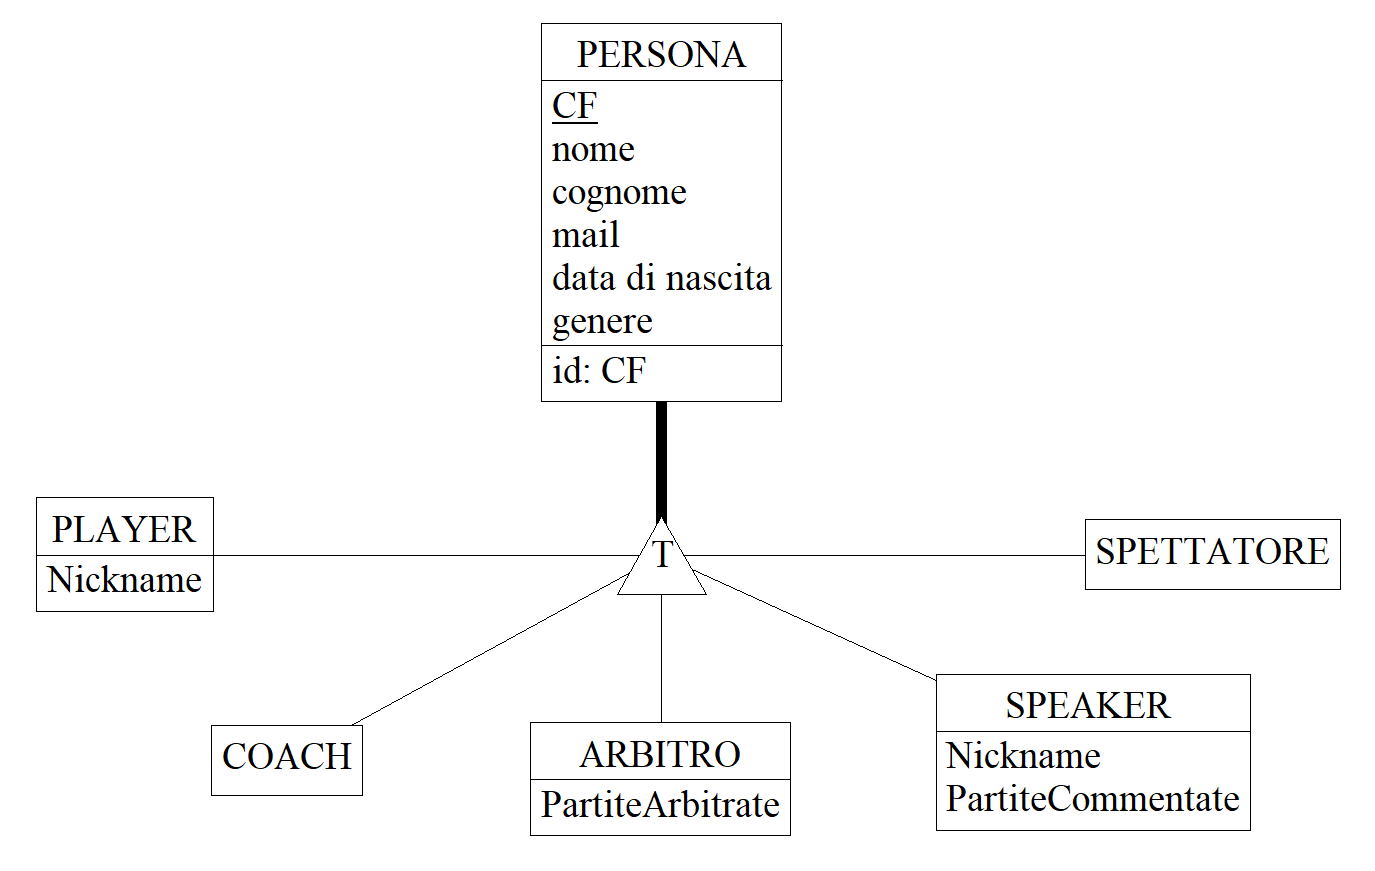
\includegraphics[scale=0.7]{img/ER_Persona.png}}
	\caption{Schema ER che espone le principali caratteristiche delle Persone}
	\label{img:ER_Persona}
\end{figure}
\section{Anteprima sviluppo dei "Videogiochi"}
bla bla bla
\begin{figure}[!htb]
	\centerline{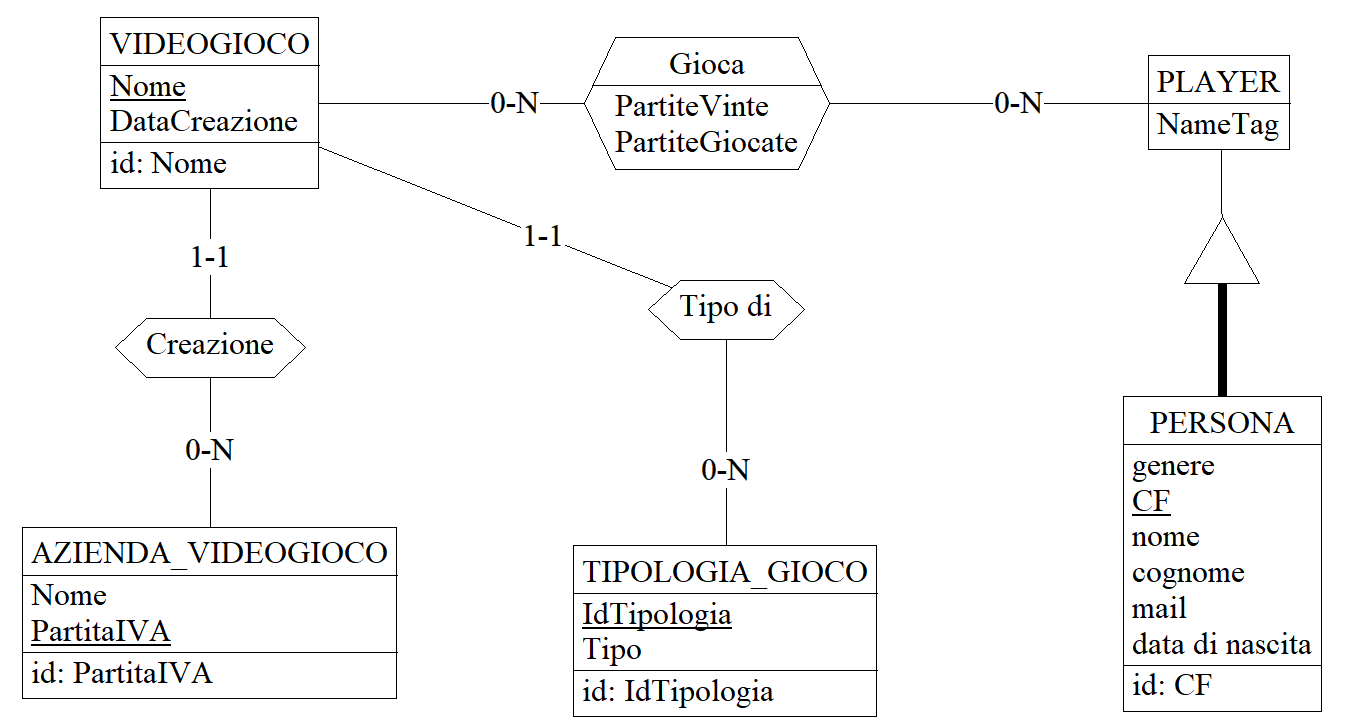
\includegraphics[scale=0.7]{img/ER_Videogiochi.png}}
	\caption{Schema ER che espone le principali caratteristiche dei Videogiochi}
	\label{img:ER_Videogiochi}
\end{figure}
\section{Anteprima sviluppo delle "Partite"}
bla bla bla
\begin{figure}[!htb]
	\centerline{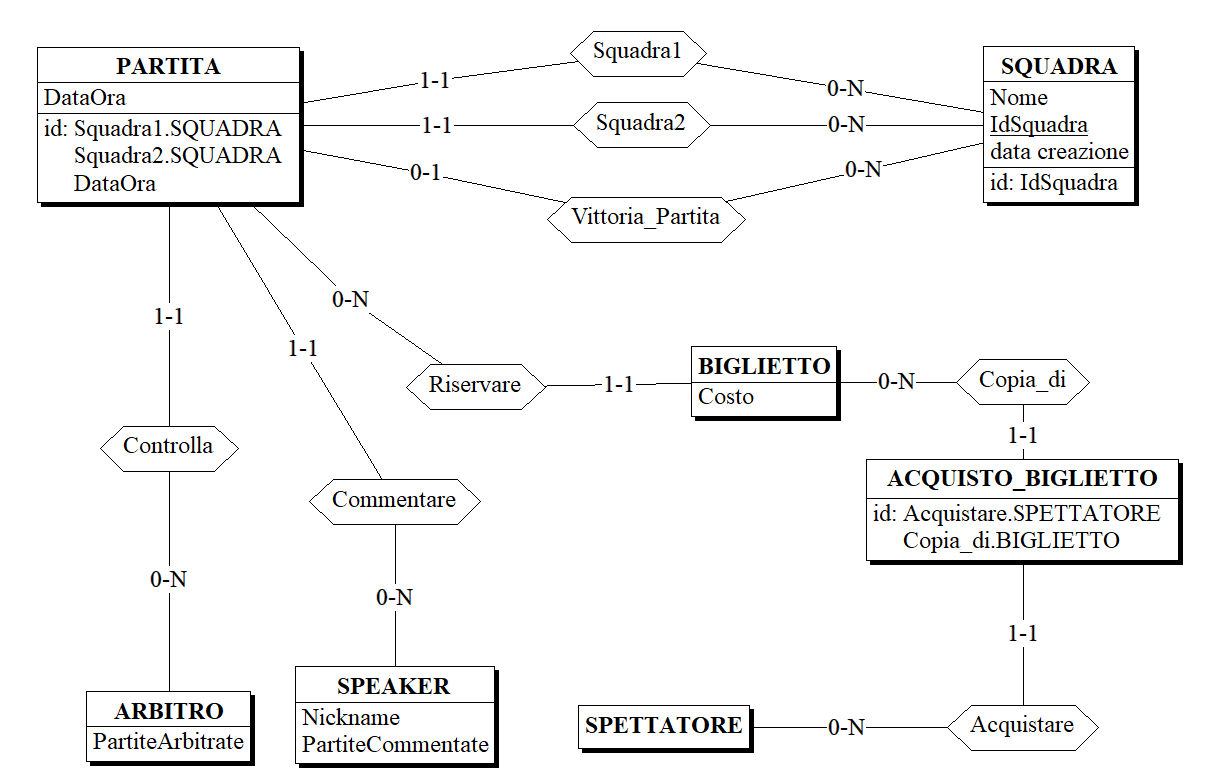
\includegraphics[scale=0.6]{img/ER_Partite.png}}
	\caption{Schema ER che espone le principali caratteristiche delle Partite}
	\label{img:ER_Partite}
\end{figure}
\section{Anteprima sviluppo dei "Tornei"}
bla bla bla
\begin{figure}[!htb]
	\centerline{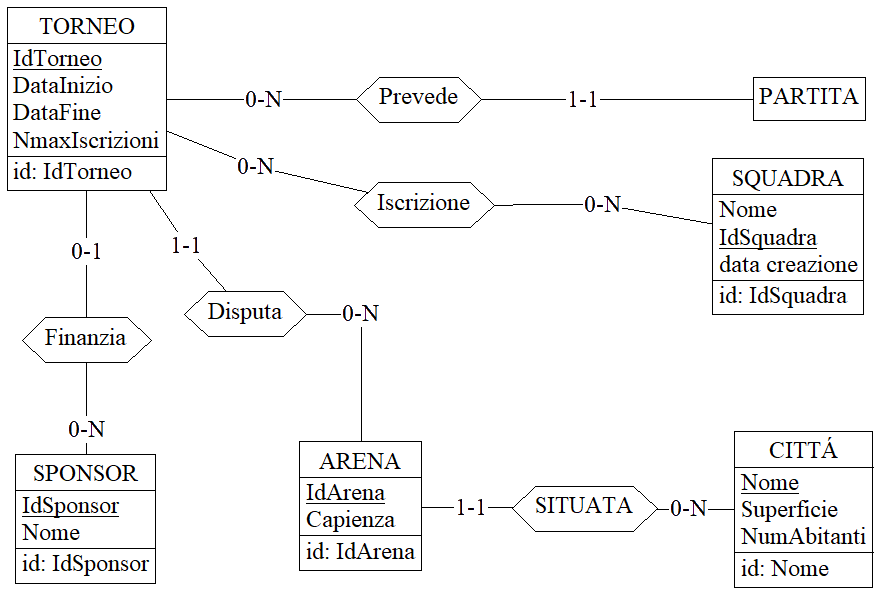
\includegraphics[scale=0.7]{img/ER_Tornei.png}}
	\caption{Schema ER che espone le principali caratteristiche dei Tornei}
	\label{img:ER_Tornei}
\end{figure}
\section{Schema Generale}
bla bla bla
\begin{figure}[!htb]
	\centerline{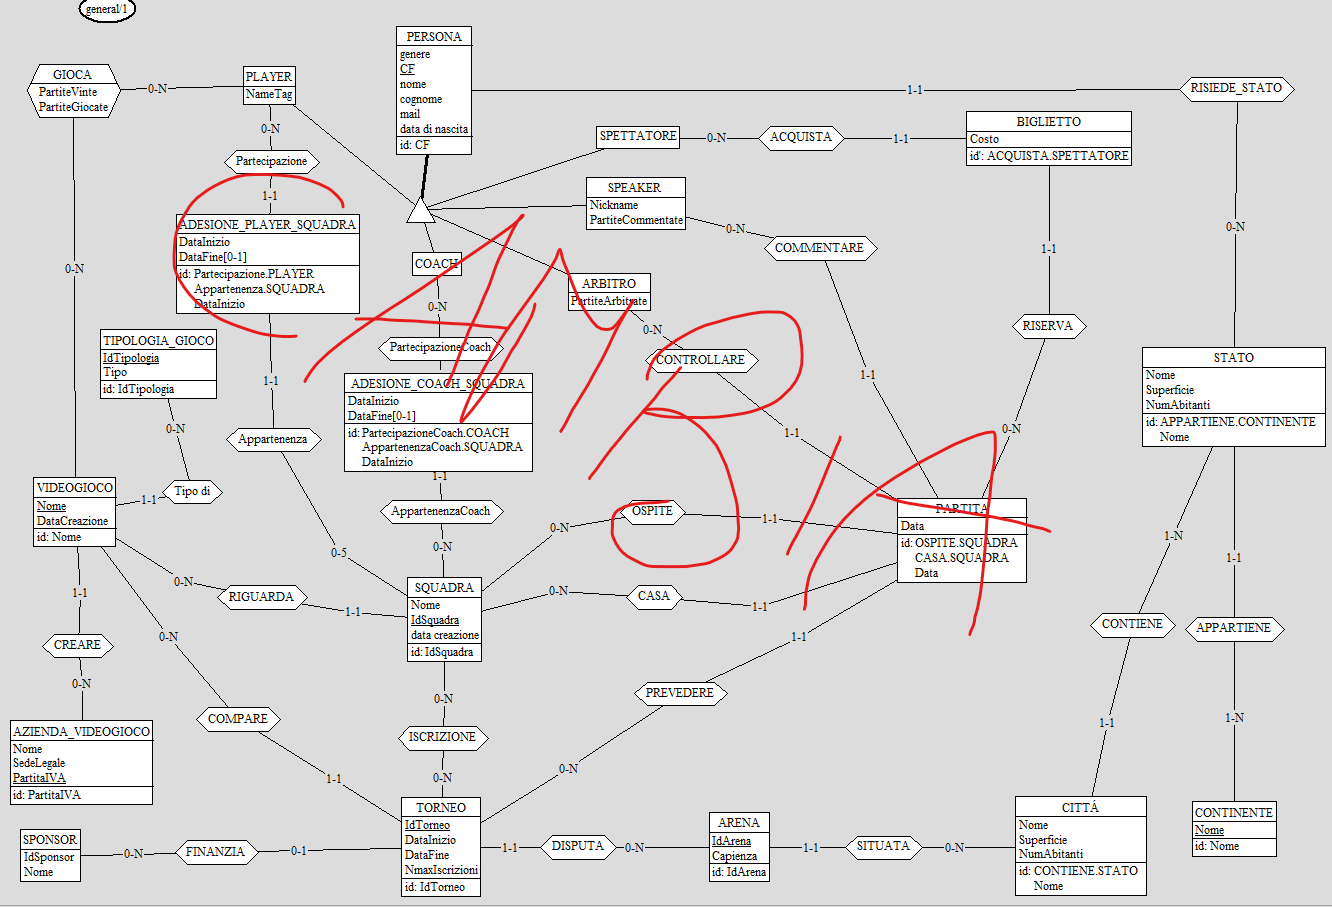
\includegraphics[scale=0.6]{img/ER_Generale.png}}
	\caption{Schema ER che espone lo schema concettuale finale}
	\label{img:ER_Generale}
\end{figure}

\chapter{Progettazione Logica}
\section{Stima del volume dei dati}
\renewcommand{\arraystretch}{1.5} %stretch scale delle celle
\setlength{\arrayrulewidth}{0.5mm}%grandezza bordi
\setlength{\tabcolsep}{10pt}%padding testo nelle celle
\setlength\doublerulesep{0.31cm}%spazio tra due linee

\begin{tabular}{|m{2cm}|c|m{2cm}|}
	\hline\rowcolor{pink}
	Soggetto & Tipo & Volume\\
	\hline\hline
	
	Player & E & 500.000\\
	\hline
	Videogiochi & E & 10\\
	\hline
	Gioca & A & 1.000.000\\
	\hline
	Azienda Videogioco & E & 5\\
	
	
	\hline
	\hline
	
	Squadra & E & 100.000\\
	\hline
	Coach & E & 50.000\\
	\hline
	Adesione Player & E & 150.000\\ 
	\hline
	Adesione Coach & E & 75.000\\ 
	
	\hline
\end{tabular}
\setlength\doublerulesep{0.18cm} %spazio tra due linee
\begin{tabular}{|m{2cm}|c|m{2cm}|}
	\hline\rowcolor{pink}
	Soggetto & Tipo & Volume\\
	\hline\hline
	Speaker & E & 1.000\\
	\hline
	Arbitro & E & 1.000\\
	\hline
	Spettatori & E & 200.000.000\\
	\hline
	Acquisto Biglietto & E & 200.000.000\\ 
	\hline
	Sponsor & E & 100\\
	
	\hline\hline
	
	Tornei & E & 10.000\\
	\hline
	Partite & E & 310.000\\
	\hline
	Previste & A & 310.000\\ 
	\hline
	Iscrizioni Torneo & A & 320.000\\ 
	\hline
	
	
\end{tabular}
\section{Descrizione delle operazioni principali e stima della loro frequenza}
Le operazioni da effettuare sono quelle già elencate nella fase di analisi. Segue una tabella
riportante la loro descrizione e relativa frequenza:
\begin{center}
	\begin{tabular}{|c|m{8cm}|c|}
		\hline\rowcolor{pink}
		Codice & Descrizione Operazione & Frequenza\\
		\hline\hline
		1 & Aggiunta di un nuovo Player & 50 al giorno\\ 
		\hline	
		2 & Aggiunta Videogioco giocato da un Player & 400 a settimana \\
		\hline
		3 & Aggiunta di un nuovo Spettatore & 30.000 a settimana \\
		\hline
		4 & Creazione di una Squadra & 100 al mese\\
		\hline 
		5 & Aggiunta di un Player ad una Squadra & 1.500 al mese\\ 
		\hline
		6 & Creazione di un Torneo & 1 a settimana\\ 
		\hline
		7 & Iscrizione di una Squadra ad un Torneo & 32 a settimana\\ 
		\hline
		8 & Creazione di nuove Partite in un Torneo & 31 a settimana\\ 
		\hline
		9 & Acquisto di un nuovo Biglietto & 30.000 a settimana\\ 
		\hline
	\end{tabular}
\end{center}
\section{Schemi di navigazione e tabelle degli accessi}
Sono riportate in seguito le tabelle degli accessi delle operazioni sopra riportate; inoltre, ove
non risulti banale, sono stati inseriti i relativi schemi di navigazione. Al fine del calcolo degli
costi, si considerano di peso doppio gli accessi in scrittura rispetto a quelli in lettura.
\renewcommand{\arraystretch}{1.15} %stretch scale delle celle
\setlength{\arrayrulewidth}{0.5mm}%grandezza bordi
\setlength{\tabcolsep}{10pt}%padding testo nelle celle
\setlength\doublerulesep{0.1cm}%spazio tra due linee
\subsection*{(1) Aggiunta di un nuovo Player}
\begin{center}
	\begin{tabular}{|c|c|c|c|}
		\hline\rowcolor{pink}
		Concetto & Costrutto & Accessi & Tipo\\
		\hline\hline
		Player & E & 1 & S\\
		\hline\hline
		\multicolumn{2}{l}{
			\textbf{Totale:} 1S * 50 al giorno → 100 al giorno} \\
		\hline
	\end{tabular}
\end{center}
\subsection*{(2) Aggiunta di un videogioco giocato da un Player}
\begin{center}
	\begin{tabular}{|c|c|c|c|}
		\hline\rowcolor{pink}
		Concetto & Costrutto & Accessi & Tipo\\
		\hline\hline
		Gioca & R & 1 & S\\
		\hline\hline
		\multicolumn{2}{l}{%
			\textbf{Totale:} 1S * 400 a settimana → 800 a settimana} \\
		\hline
	\end{tabular}
\end{center}
\subsection*{(3) Aggiunta di un nuovo Spettatore}
\begin{center}
	\begin{tabular}{|c|c|c|c|}
		\hline\rowcolor{pink}
		Concetto & Costrutto & Accessi & Tipo\\
		\hline\hline
		Spettatore & E & 1 & S\\
		\hline\hline
		\multicolumn{2}{l}{%
			\textbf{Totale:}  1S * 30.000 a settimana → 60.000 a settimana } \\
		\hline
	\end{tabular}
\end{center}
\subsection*{(4) Creazione di una Squadra}
\begin{center}
	\begin{tabular}{|c|c|c|c|}
		\hline\rowcolor{pink}
		Concetto & Costrutto & Accessi & Tipo\\
		\hline
		Squadra & E & 1 & S\\
		\hline\hline
		\multicolumn{2}{l}{%
			\textbf{Totale:} 1S * 100 al mese  → 200 al mese} \\
		\hline\hline
	\end{tabular}
\end{center}
\subsection*{(5) Aggiunta di un Player ad una Squadra}
controllo la squadra se gia piena e ce lo caccio dentro
\begin{center}
	\begin{tabular}{|c|c|c|c|}
		\hline\rowcolor{pink}
		Concetto & Costrutto & Accessi & Tipo\\
		\hline\hline		
		Squadra & E & 1 & L\\
		Adesione Player & A & 1 & S\\
		\hline
		\hline
		\multicolumn{2}{l}{%
			\textbf{Totale:} (1L + 2S) * 150.000 al giorno → 450.000 al giorno} \\
		\hline
	\end{tabular}
\end{center}
\subsection*{(6) Creazione di un Torneo}
\begin{center}
	\begin{tabular}{|c|c|c|c|}
		\hline\rowcolor{pink}
		Concetto & Costrutto & Accessi & Tipo\\
		\hline\hline		
		Torneo & E & 1 & S\\
		Arena & E & 1 & L\\
		Partite Previste & A & 31 & S\\
		Iscrizione Squadra & A & 32 & S\\
		\hline
		\hline
		\multicolumn{2}{l}{%
			\textbf{Totale:} (1S + 1L + 31S + 32S) → 129 alla settimana} \\
		\hline
	\end{tabular}
\end{center}
\subsection*{(7) Iscrizione di una Squadra ad un Torneo}
\begin{center}
	\begin{tabular}{|c|c|c|c|}
		\hline\rowcolor{pink}
		Concetto & Costrutto & Accessi & Tipo\\
		\hline\hline		
		Torneo & E & 1 & L\\
		Iscrizione Squadra & A & 1 & S\\
		\hline
		\hline
		\multicolumn{2}{l}{%
			\textbf{Totale:} (1L + 1S) * 32 a settimana → 96 a settimana} \\
		\hline
	\end{tabular}
\end{center}
\subsection*{(8) Creazione di nuove Partite in un Torneo}
\begin{center}
	\begin{tabular}{|c|c|c|c|}
		\hline\rowcolor{pink}
		Concetto & Costrutto & Accessi & Tipo\\
		\hline\hline		
		Partita & E & 1 & S\\
		Partita Prevista & A & 1 & S\\
		Torneo & E & 1 & L\\
		\hline
		\hline
		\multicolumn{2}{l}{%
			\textbf{Totale:} (1L + 2S + 2S) * 31 a settimana → 155 a settimana} \\
		\hline
	\end{tabular}
\end{center}
\subsection*{(9) Acquisto di un nuovo Biglietto}
\begin{center}
	\begin{tabular}{|c|c|c|c|}
		\hline\rowcolor{pink}
		Concetto & Costrutto & Accessi & Tipo\\
		\hline\hline		
		cambiare & E & 1 & L\\
		cambiare & A & 1 & S\\
		\hline
		\hline
		\multicolumn{2}{l}{%
			\textbf{Totale:} 1L + 2S → 450.000} \\
		\hline
	\end{tabular}
\end{center}
\section{Raffinamento dello schema}
\subsection{Eliminazione Gerarchie}
\subsection{Eliminazione attributi composti}
\subsection{Scelta delle Chiavi}
\section{Analisi delle ridondanze}
\section{Traduzione di entità e associazioni in relazioni}
\section{Schema relazionale finale}


\chapter{Progettazione Fisica}
\section{Traduzione in SQL}


\chapter{Progettazione dell'Applicazione}
\section{Descrizione della scelta del linguaggio e del DBMS}
\section{Descrizione dell'architettura}
\section{Interfaccia Utente}
\subsection{Amministratore Torneo}
\subsection{Giocatore}
\end{document}
